\section*{Exercice 170 -- SLCI Calculs}
% CCP MP 2012

\setcounter{exo}{0}


Soient les schéma-blocs suivants. 
\begin{center}
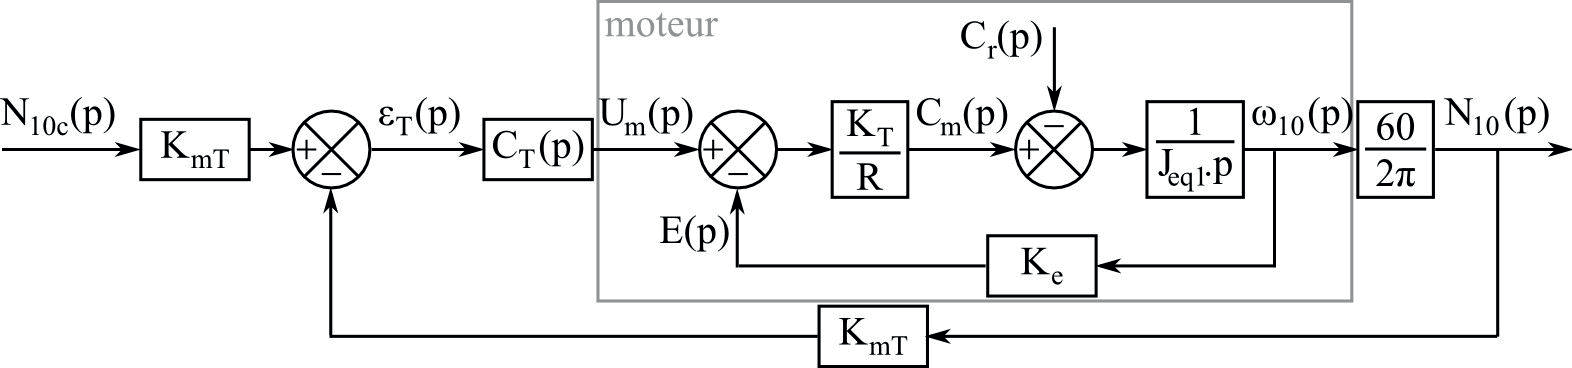
\includegraphics[width=1.0\linewidth]{046_01.png}
\end{center}



\begin{center}
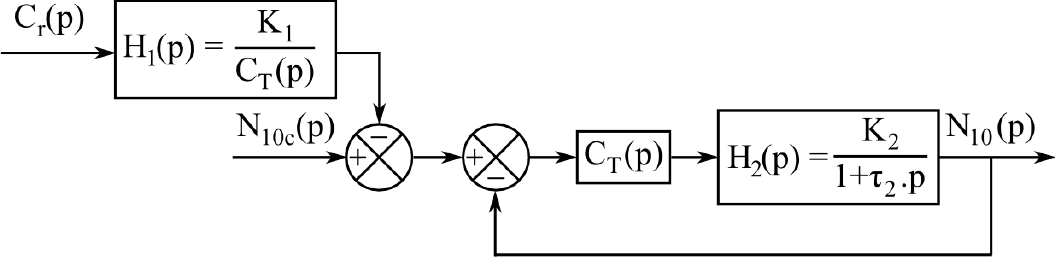
\includegraphics[width=1.0\linewidth]{046_02.png}
\end{center}



\subparagraph{}\textit{Mettre le premier schéma-blocs sous la forme du second schéma-blocs. Exprimer les fonctions de transfert $H_1(p)$ et $H_2(p)$ en fonction des paramètres du premier schéma-blocs.}
\ifprof
\begin{corrige}
\end{corrige}
\else
\fi